\documentclass[text05.tex]{subfiles}
\begin{document}
\subsubsection{スイッチ}\label{switch}
\begin{table}[H]
  \begin{widerrows}
    \begin{tabular}{|p{\colF}|p{\colG}|}	\hline
    \ruby{名称}{めい|しょう} & スイッチ（すいっち）\\ \hline
    \ruby{接続箇所}{せつ|ぞく|か|しょ} & デジタルコネクタ (3pin)\\ \hline
    \ruby{機能概要}{き|のう|がい|よう} & ONとOFFを切りかえる\\ \hline
    \end{tabular}
  \end{widerrows} 
\end{table}

\begin{table}[H]
  \begin{widerrows}
    \begin{tabular}{|p{\colF}|p{\colG}|}	\hline
    サンプルコードの場所 & 05/digin.hsp\\ \hline
    raspiへの入力 & 右にスライドさせると１、左にスライドさせると０を入力する\\ \hline
    raspiへの入力方法 & val = gpioin(GPIO番号)\\ \hline
    raspiからの出力 & なし\\ \hline
    raspiからの出力方法 & なし\\ \hline
    \end{tabular}
  \end{widerrows} 
\end{table}

\begin{table}[H]
  \begin{widerrows}
    \begin{tabular}{|p{\colF}|p{\colG}|} \hline
    使い道 & 照明のスイッチ\\ \hline
    \ruby{注意事項}{ちゅう|い|じ|こう} & なし\\ \hline
    \ruby{補足}{ほ|そく} & ボタンと\ruby{違}{ちが}い、人の手を使わなくとも\ruby{値}{あたい}を\ruby{保持}{ほ|じ}しておくことができます。\\ \hline
    \end{tabular}
  \end{widerrows} 
\end{table}

\begin{figure}[H]
  \begin{widerrows}
    \begin{tabular}{|p{\colH}|p{\colI}|p{\colH}|p{\colI}|} \hline
    外観 & 
    \begin{minipage}[t]{\linewidth}
      \smallskip
        \centering
        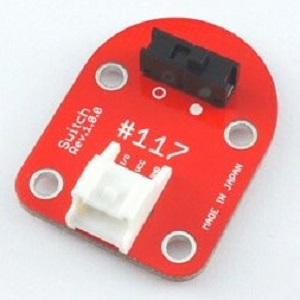
\includegraphics[width=0.5\linewidth]{../../asset/image/text05-img019.jpg}
        \caption{スイッチ}
        \smallskip
      \end{minipage} &
      回路記号 & 
      \begin{minipage}[t]{\linewidth}
      \smallskip
        \centering
        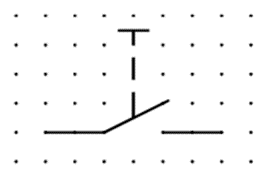
\includegraphics[width=0.5\linewidth]{../../asset/image/text05-img047.png}
        \caption{スイッチの回路図}
        \smallskip
      \end{minipage}\\ \hline
    \end{tabular}
  \end{widerrows} 
\end{figure}\end{document}
